\section{Richiami di ottica}

Il comportamento dei raggi di luce viene descritto dalla cosiddetta ottica
geometrica. L'ottica geometrica è solo una approssimazione del comportamento
della luce, che viene descritto completamente dall'ottica ondulatoria, ma una
approssimazione che è in grado di descrivere la maggior parte dei
fenomeni.Nell'ottica geometrica, la luce è formata da raggi che si propagano
in linea retta in un mezzo. Ogni mezzo è caratterizzato da un numero chiamato
indice di rifrazione ($n$). L'indice di rifrazione dipende dalla composizione
e dalla densità del mezzo. Nella tabella \ref{table:indici-rifrazione} sono



\begin{figure}[!ht]
\begin{subfigure}[t]{.5\textwidth}
\centering
\caption{Riflessione}
\label{sub:riflessione}
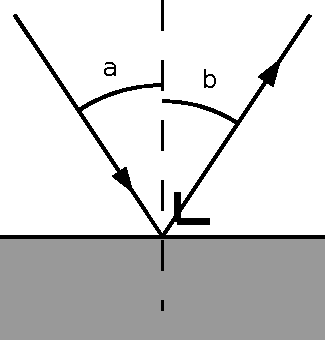
\includegraphics[height=3cm]{img/riflessione.pdf}

\end{subfigure}
\begin{subfigure}[t]{.5\textwidth}
\caption{Rifrazione}
\label{sub:rifrazione}
\centering
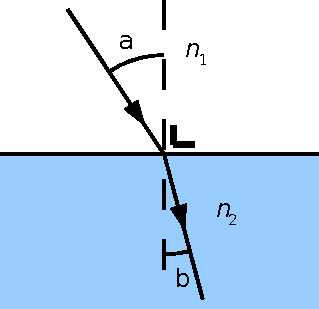
\includegraphics[height=3cm]{img/rifrazione.pdf}


\end{subfigure}
\caption{Riflessione e rifrazione}
\label{fig:riflessione-rifrazione}
\end{figure}


Quando i raggi incontrano una superficie che separa due mezzi con diversi
indici di rifrazione (ad esempio aria e vetro, oppure aria ed acqua, o anche
due vetri diversi), il comportamento dei raggi di luce è regolato da due leggi
fondamentali:

\begin{enumerate}
\item Nella riflessione (Figura \ref{fig:riflessione-rifrazione} -- \subref{sub:riflessione}) il raggio di luce (detto incidente) dà origine ad un raggio riflesso. L'angolo incidente è uguale all'angolo riflesso misurato rispetto alla perpendicolare della superficie. La
riflessione avviene in modo pressoché completo solo in alcuni casi, di solito quando si ha a che fare
con una superficie metallica.
\item Nella rifrazione (Figura \ref{fig:riflessione-rifrazione} -- \subref{sub:rifrazione}) il raggio di luce incidente dà origine a un raggio rifratto. Anche qui
consideriamo gli angoli rispetto alla perpendicolare della superficie, e la loro relazione è regolata
dalla cosiddetta legge di Snell.
\end{enumerate}


\begin{table}
\centering
\begin{tabular}{l|c}

Mezzo & Indice di rifrazione ($n$) \\
\hline
Vuoto &1\\
Aria  &1,00029\\
Acqua &1,333\\
Plexiglas &1,49\\
Vetro crown &1,51-1,61\\
Vetro flint &1,51-1,89\\
Diamante &2,417\\
\end{tabular}

\caption{Indici di rifrazione}
\label{table:indici-rifrazione}

\end{table}

\subsection{Rifrazione - legge di Snell}


La rifrazione è la deviazione subita da un'onda che ha luogo quando questa
passa da un mezzo ad un altro  nel quale la sua velocità di propagazione
cambia. La legge di Snell, nota anche come legge di Descartes o legge di
Snell-Descartes (o legge di Cartesio o legge di Snell-Cartesio), descrive le
modalità di rifrazione di un raggio luminoso nella transizione tra due mezzi
con indice di rifrazione diverso, e deriva dall'equazione iconale. La figura
\ref{fig:snell} mostra due mezzi trasmissivi con indice di rifrazione $n_1$ (a
sinistra) e $n_2$ (a destra) in contatto tra loro attraverso una superficie,
che viene chiamata interfaccia (linea verticale in figura). Nel caso $n_2 >
n_1$, la luce ha una velocità di fase più bassa nel secondo mezzo. Il raggio
luminoso $PO$ proveniente dal mezzo di sinistra colpisce l'interfaccia nel
punto $O$. A partire da tale punto $O$ tracciamo una retta perpendicolare
all'interfaccia stessa, che viene chiamata normale all'interfaccia (linea
orizzontale in figura). L'angolo tra la normale e il raggio luminoso $PO$
viene chiamato angolo d'incidenza, $\theta_1$. Il raggio attraversa
l'interfaccia e prosegue nel mezzo di destra, indicato come $OQ$. L'angolo che
tale raggio (rifratto) forma con la normale si chiama angolo di rifrazione,
$\theta_2$. La legge di Snell fornisce la relazione tra gli angoli $\theta_1$
e $\theta_2$: 
\[n_1 \sin(\theta_1)=n_2 \sin(\theta_2)\]
 Si noti che nel caso
$\theta_1 = 0\degree$ (ovvero il raggio risulta perpendicolare
all'interfaccia) la soluzione è $\theta_2 = 0\degree$ per qualunque valore di
$n_1$ e $n_2$. In altri termini, un raggio che entra in un mezzo in modo
perpendicolare alla sua superficie non viene mai deviato. Quanto detto sopra
vale anche nel caso di un raggio luminoso che passa da un mezzo più denso a
uno meno denso; la simmetria della legge di Snell mostra che gli stessi
percorsi luminosi sono validi anche nella direzione opposta. Una regola di
carattere qualitativo per determinare la direzione della rifrazione è che il
raggio luminoso è sempre più vicino alla normale dal lato del mezzo più denso.
La legge di Snell è valida in generale solo per mezzi isotropi, come il vetro.
Nel caso di mezzi anisotropi (ad esempio alcuni cristalli) il fenomeno della
birifrangenza può dividere in due il raggio rifratto. Si vengono allora ad
avere due raggi, uno ordinario (raggio o) che segue la legge di Snell, e uno
straordinario (raggio e) che può non essere complanare con quello incidente.

\begin{figure}
\centering
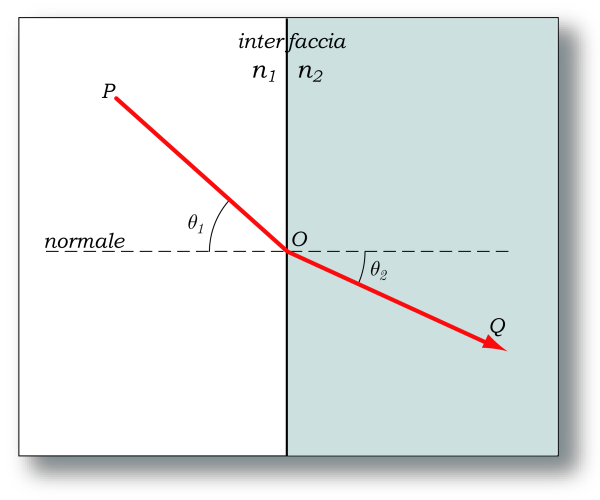
\includegraphics[width=.5\textwidth]{img/Legge_di_Snell.png}
\caption{Rifrazione}\label{fig:snell}
\end{figure}

\subsection{Riflessione} 

La riflessione è il fenomeno per cui un'onda, che si propaga lungo
l'interfaccia tra differenti mezzi, cambia di direzione a causa di un impatto
con un materiale riflettente. Assorbimento, riflessione e trasmissione sono i
fenomeni che avvengono quando la luce interagisce con la materia. Quando
l'energia radiante incide su un corpo, una parte viene assorbita, una parte
viene riflessa e una parte viene trasmessa. Per la legge di conservazione
dell'energia, la somma delle quantità di energia rispettivamente assorbita,
riflessa e trasmessa è uguale alla quantità di energia incidente. Per indicare
il tipo di riflessione di cui si tratta si usano gli aggettivi:

\begin{itemize}

\item Spettrale: per indicare la radiazione monocromatica, cioè considerata
lunghezza d'onda per lunghezza d'onda; 

\item Radiante (contrapposto a luminosa): per indicare che la radiazione è
data in termini di energia totale, cioè è espressa mediante grandezze
radiometriche;

\item Luminosa (contrapposto a radiante): per indicare che la radiazione è
pesata secondo la funzione di efficienza luminosa dell'occhio, cioè è espressa
in grandezze fotometriche; 

\end{itemize}
\begin{figure}[!bh]
\begin{subfigure}[b]{.5\textwidth}
\centering
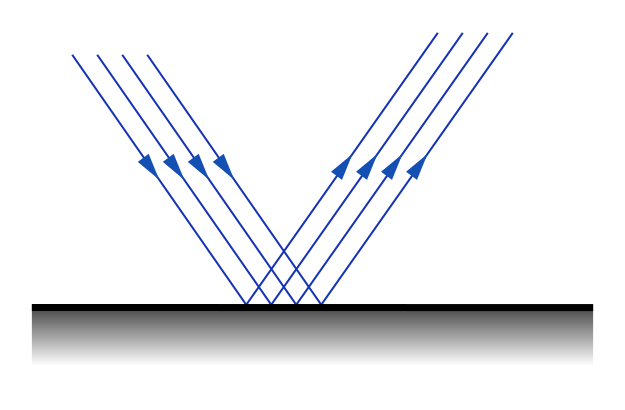
\includegraphics[height=4cm]{img/riflessione.png}
\caption{Riflessione Speculare}\label{fig:riflessione1}
\end{subfigure}
\begin{subfigure}[b]{.5\textwidth}
\centering
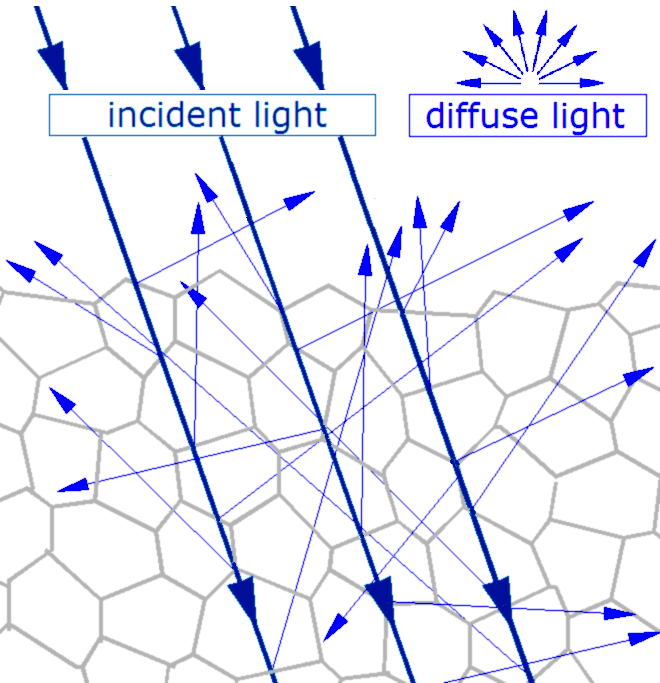
\includegraphics[height=4cm]{img/riflessione_diffusa.png}
\caption{Riflessione Diffusa}\label{fig:riflessione2}
\end{subfigure}
\end{figure}
La riflessione può avvenire:
\begin{itemize}
\item Specularmente (riflessione speculare o regolare) cioè in una unica (o quasi) direzione
\item Diffusamente (riflessione diffusa) cioè in varie direzioni;
\end{itemize}
La riflettanza (reflectance) è il rapporto tra flusso riflesso e flusso
incidente valutato per ogni lunghezza d'onda. Essendo definita come rapporto
di grandezze omogenee, la riflettanza è una grandezza adimensionale e viene
espressa in percentuale (0-100\%) o come fattore (0.0-1.0). Inoltre riguarda
il flusso e quindi la totalità della radiazione riflessa nella emisfera. La
riflettanza non è solo funzione della lunghezza d'onda ma anche
dell'illuminazione, della geometria di irradiamento e della geometria di
visione (cioè della geometria con cui si illumina il corpo e della geometria
con cui si misura la quantità riflessa), per cui è necessario definire una
grandezza più generale della riflettanza, cioè il fattore di riflessione. Si
fa riferimento al diffusore riflettente ideale. Si tratta di un corpo (ideale,
cioè teorico) che non assorbe e non trasmette, ma riflette diffusamente la
radiazione ricevuta con radianza o luminanza uguale per ogni angolo di
riflessione e indipendentemente dalla direzione della radiazione incidente.
Come prima applicazione del concetto di diffusore riflettente ideale si
definisce il fattore di radianza (radiance factor) o il fattore di luminanza
(luminance factor) come il rapporto tra la radianza di un'area e quella del
diffusore ideale riflettente irradiato nello stesso modo. Con riferimento a
questo corpo ideale, il fattore di riflessione (reflectance factor o
reflection factor) di un corpo è il rapporto tra il flusso riflesso dal corpo
in un dato cono il cui vertice è sul corpo considerato e il flusso riflesso
dal diffusore riflettente ideale. Il fattore di riflessione è dunque una
grandezza generica che corrisponde: alla riflettanza spettrale se il cono è
una emisfera; al fattore di radianza spettrale se il cono è stretto. Un tipico
spettrofotometro è in grado di misurare il fattore di riflessione spettrale ad
intervalli di 10 nm nell'intervallo da 380 a 730 nm. La riflessione di onde
elettromagnetiche è regolata da due leggi fondamentali, ricavabili dal
principio di Fermat e dal principio di Huygens-Fresnel:

\begin{itemize}
\item Il raggio incidente, il raggio riflesso e la normale al piano nel punto
di incidenza giacciono sullo stesso piano;
\item L'angolo di incidenza e l'angolo di riflessione sono uguali;
\end{itemize}

Un'onda elettromagnetica riflessa può subire uno sfasamento. Questo dipende
dagli indici di rifrazione del mezzo nel quale viaggia la luce ($n1$) e del
mezzo oltre la superficie riflettente ($n2$):

\begin{tabular}{l}
se $n1>n2$ non c'è sfasamento;\\
se $n1<n2$ la radiazione riflessa è sfasata di $\pi$, cioè di mezza lunghezza d'onda.\\
\end{tabular}


\subsection{Lenti}
Una lente è un elemento ottico che ha la proprietà di concentrare o di far divergere i raggi di luce. Grazie a questa proprietà può formare immagini, reali o \emph{virtuali}, di oggetti.
Normalmente è realizzata in vetro o materiali plastici. Esistono anche dispositivi analoghi, che operano su altre bande dello spettro elettromagnetico o altre forme di radiazione, comunque chiamati lenti.

Una lente convergente (Figura \ref{fig:lenti} -- \subref{fig:lente-convergente})
 sfrutta la rifrazione per convogliare i raggi provenienti da un
punto oggetto in un altro punto detto fuoco. Le superfici sono opportunamente
sagomate, solitamente in forma sferica, per raggiungere questo scopo. Il
risultato è la creazione di una immagine i cui punti corrispondono ai punti
dell'oggetto osservato (Figura \ref{fig:formazione-immagine} -- \subref{fig:formazione-lente-convergente}). L'immagine può essere osservata su uno schermo
posto sul suo piano, oppure raccolta con una pellicola o anche osservata ad
occhio nudo. Se l'oggetto si trova all'infinito, come nel caso di un oggetto
astronomico, la distanza tra la lente e l'immagine ($d_2$) è pari alla
lunghezza focale. Altrimenti vale la formula:   \[ \frac{1}{d_1} +
\frac{1}{d_2} = \frac{1}{f} \] dove $d_1$ è la distanza tra l'oggetto e la
lente, $d_2$ è la distanza tra la lente e l'immagine e $f$ è la lunghezza
focale.

In una lente divergente (Figura \ref{fig:lenti} -- \subref{fig:lente-divergente}),
i raggi di luce non convergono, ma se li prolunghiamo dalla
parte della lente troviamo che si radunano comunque in un punto, che chiamiamo
fuoco virtuale. In questo modo si forma (Figura \ref{fig:formazione-immagine} -- \subref{fig:formazione-lente-divergente}) una immagine virtuale, che può
essere osservata guardando attraverso la lente, ma che non può essere raccolta
su uno schermo.


\begin{figure}
\begin{subfigure}[b]{.5\textwidth}
\centering
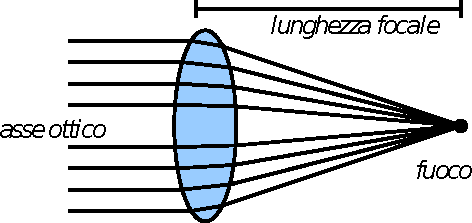
\includegraphics[height=3cm]{img/lente-convergente.pdf}
\caption{Lente convergente}\label{fig:lente-convergente}
\end{subfigure}
\begin{subfigure}[b]{.5\textwidth}
\centering
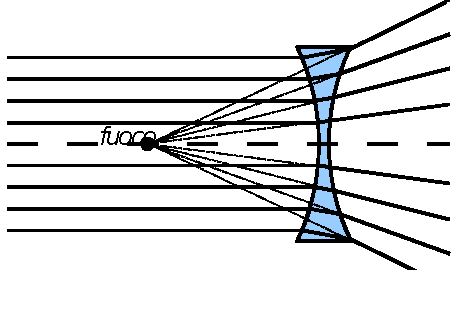
\includegraphics[height=3cm]{img/lente-divergente.pdf}
\caption{Lente divergente}\label{fig:lente-divergente}
\end{subfigure}
\caption{Lenti}
\label{fig:lenti}
\end{figure}

\begin{figure}
\begin{subfigure}[b]{.5\textwidth}
\centering
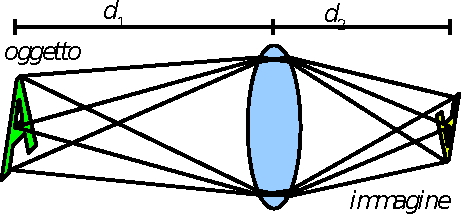
\includegraphics[height=3cm]{img/formazione-immagine.pdf}
\caption{Lente convergente}\label{fig:formazione-lente-convergente}
\end{subfigure}
\begin{subfigure}[b]{.5\textwidth}
\centering
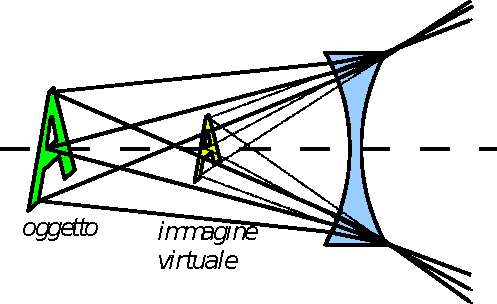
\includegraphics[height=3cm]{img/formazione-immagine-divergente.pdf}
\caption{Lente divergente}\label{fig:formazione-lente-divergente}
\end{subfigure}
\caption{Formazione dell'immagine}
\label{fig:formazione-immagine}
\end{figure}

\subsection{Gli specchi}

Uno specchio è formato da un substrato di vetro o altro materiale su cui viene depositato un sottile
strato di alluminio seguito da altre sostanze per incrementarne la resistenza o la riflettività. Lo
specchio più semplice è quello sferico, tuttavia  usato per osservare oggetti a
grande distanza presenta il difetto detto aberrazione sferica,  i raggi riflessi nelle zone
periferiche dello specchio vengono focalizzati più vicino rispetto a quelli riflessi nelle zone centrali
(Figura \ref{fig:specchi} -- \subref{fig:specchio-sferico}).
Lo specchio può essere anche un paraboloide (Figura \ref{fig:specchi} -- \subref{fig:specchio-parabolico}), nel qual caso lo specchio viene detto parabolico. 
L'aberrazione sferica può essere corretta utilizzando un sistema  complesso di specchi o di specchi e lenti, in cui l'aberrazione introdotta da un componente viene corretta dagli altri.
Come per una lente, anche per uno specchio viene definita una lunghezza focale che corrisponde
alla distanza tra il centro dello specchio e il fuoco.

\begin{figure}
\begin{subfigure}[b]{.5\textwidth}
\centering
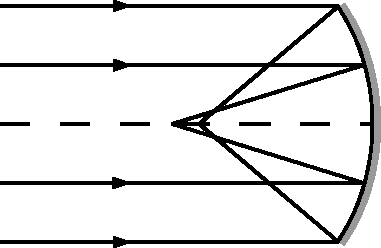
\includegraphics[height=3cm]{img/specchio-sferico.pdf}
\caption{Specchio sferico}\label{fig:specchio-sferico}
\end{subfigure}
\begin{subfigure}[b]{.5\textwidth}
\centering
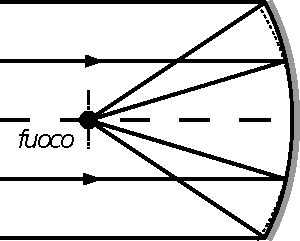
\includegraphics[height=3cm]{img/specchio-parabolico.pdf}
\caption{Specchio parabolico}\label{fig:specchio-parabolico}
\end{subfigure}
\caption{Specchi}
\label{fig:specchi}
\end{figure}


\begin{figure}

\centering
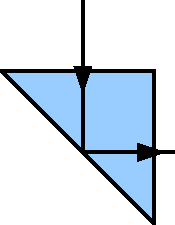
\includegraphics[height=3cm]{img/diagonale-prisma.pdf}

\caption{Prisma diagonale}
\label{fig:specchio-diagonale}
\end{figure}


\subsection{Approssimazione parassiale} 
Nell'ottica geometrica si può applicare l'approssimazione parassiale quando
tutti i raggi che entrano o escono da un sistema ottico centrato si propagano
dal piano oggetto al piano immagine ad angoli piccoli rispetto all'asse del
sistema, rimanendo quindi confinati in una regione prossima all’asse ottico
("parassiale"). In questo caso, si dice che il sistema ottico forma l’immagine
dell’oggetto in condizioni parassiali.

In approssimazione parassiale, quindi, nella legge di Snell si può
approssimare il seno con il suo argomento (e il coseno con 1), dato che gli
angoli di incidenza, di riflessione e di rifrazione sono piccoli.

Una lente sferica semplice dà un'immagine (monocromatica) correttamente messa
a fuoco, reale o virtuale, solo se è in condizioni parassiali, cioè se
l'oggetto è visto con un angolo piccolo e se il diametro della lente è piccolo
rispetto alla distanza focale e alla distanza dell'oggetto. Al crescere degli
angoli nascono aberrazioni.

\subsection{Aberrazione}
L'aberrazione di un sistema ottico è la differenza tra l'immagine effettiva,
reale o virtuale, formata dal sistema e l'immagine che si voleva ottenere,
immagine che di solito è bidimensionale e consiste in una proiezione
geometrica della scena reale sul piano focale del sistema secondo i principi
dell'ottica geometrica ideale. Le aberrazioni possono dare scarsa nitidezza,
deformazioni dell'immagine, differenze tra le immagini corrispondenti ai
diversi colori, non uniformità della luminosità.

In particolare, si chiamano aberrazioni le differenze di un'immagine rispetto
a quella previste in approssimazione parassiale. Si distinguono le aberrazioni
policromatiche (dovute alla dipendenza dell'indice di rifrazione dalla
lunghezza d'onda della luce) da quelle monocromatiche.

Le aberrazioni ricadono in due classi:
\begin{itemize}
	\item Monocromatiche: causate dalla geometria delle lenti o degli specchi, si verificano sia quando la luce è riflessa, sia quando è rifratta, si verificano anche utilizzando luce monocromatica (il cui contenuto è un unica lunghezza d'onda).
	\item Cromatiche: sono causate dalla dispersione, la variazione dell'indice di rifrazione in funzione della lunghezza d'onda, non si verificano in caso di luce monocromatica.
\end{itemize}
Consideriamo adesso alcune aberrazioni partendo dalle legge di snell:
\[\sin(\theta_1)=\frac{n_2}{n_1 } \sin(\theta_2)\]
e avvalendoci di uno sviluppo consideriamo una teoria del terzo ordine:
\[\sin(\theta) \simeq \theta - \frac{\theta^3}{3}\]
In questo caso si identificano 5 aberrazioni monocromatiche:
\begin{enumerate}
\item Aberrazione sferica
\item Coma
\item Astigmatismo
\item Curvatura di campo
\item Distorsione
\end{enumerate}

\subsection{Aberrazione Sferica} 

L'aberrazione sferica è propria dei sistemi ottici con lenti sferiche. Questo
tipo di aberrazione è provocato dal fatto che la sfera non è la superficie
ideale per realizzare una lente, ma è comunemente usata per semplicità
costruttiva. I raggi distanti dall'asse vengono focalizzati ad una distanza
differente dalla lente rispetto a quelli più centrali. Per evitare il fenomeno
si utilizzano particolari lenti non sferiche, chiamate asferiche, più
complesse da realizzare e molto costose. Il difetto può anche essere
minimizzato scegliendo opportunamente il tipo di lente adatto all'impiego
specifico; per esempio una lente piano-convessa è adatta per focalizzare un
fascio collimato a formare un punto preciso, se usata con il lato convesso
rivolto verso il fascio.

\begin{figure}

\centering
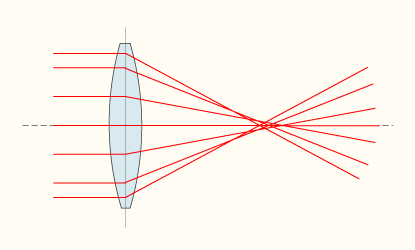
\includegraphics[width=.5\textwidth]{img/aberrazione-sferica.png}

\caption{Aberrazione sferica}
\label{fig:astigmatismo}
\end{figure}

\subsection{Coma}  
La coma è un'aberrazione ottica che deriva il suo nome dal caratteristico
aspetto a cometa delle immagini create dai sistemi ottici che presentano tale
difetto. La coma si ha quando l'oggetto ripreso è spostato lateralmente
rispetto all'asse del sistema di un angolo $\theta$. I raggi che passano per il
centro di una lente con distanza focale $f$, sono focalizzati alla distanza $f \tan(\theta)$.
I raggi che passano in periferia sono focalizzati invece in un punto
diverso sull'asse, più lontano nel caso della coma positiva e più vicino nella
coma negativa. In generale, un fascio di raggi passanti per la lente ad una
certa distanza dal centro, è focalizzato in una forma ad anello sul piano
focale. La sovrapposizione di questi diversi anelli origina una forma a V,
simile alla coda di una cometa (da cui il nome: in Latino coma = chioma). Come
per l'aberrazione sferica, la coma può essere ridotta (e in alcuni casi
eliminata) scegliendo opportunamente la curvatura delle lenti in funzione
dell'uso.

\begin{figure}

\centering
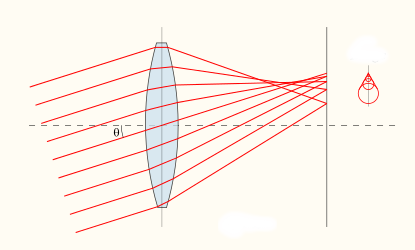
\includegraphics[width=.5\textwidth]{img/coma.png}

\caption{Coma}
\label{fig:coma}
\end{figure}

\subsection{Astigmatismo}

L'astigmatismo è un'aberrazione ottica presente in un sistema singolo o
composto di lenti, dagli obbiettivi all'occhio; i raggi che si propagano in
due piani intersecanti l'asse ottico ad angoli diversi, ad esempio
perpendicolari tra loro, hanno fuochi differenti e proiettando l'immagine di
un punto, lo stesso risulta deformato. Se un sistema ottico con astigmatismo
viene utilizzato per formare l'immagine di una croce, le linee orizzontali e
verticali saranno a fuoco a due distanze diverse. Visivamente un'immagine
prodotta da un sistema astigmatico apparirà più o meno evidentemente deformata
(un punto risulterà ellittico, con parte del bordo sfocato) o sdoppiata], con
un'immagine principale a fuoco ed una secondaria, meno incisa, sfocata e
traslata rispetto a quella principale, a renderne meno intelligibile la
lettura. L'aberrazione colpisce potenzialmente tutti i sistemi ottici ed è
particolarmente sentita nei telescopi rifrattivi e nei microscopi  per
l'importanza estrema del dettaglio.

L'astigmatismo assiale e sagittale costituisce una delle cinque aberrazioni
primarie di Seidel o aberrazioni primarie monocromatiche. Sul piano di Gauss
la figura descritta dalle equazioni di Seidel per l'aberrazione astigmatica e
di curvatura di campo (un sistema di equazioni in genere espresse in
coordinate polari) è un’ellisse parametrizzata da fattori tra cui i
coefficienti di aberrazione che modificano le sue dimensioni (entità
dell'aberrazione) e la sua forma. Quando La curvatura di campo è uguale a 0 si
ha l’astigmatismo sagittale puro, nel caso opposto si ha l’astigmatismo
tangenziale.

\begin{figure}

\centering
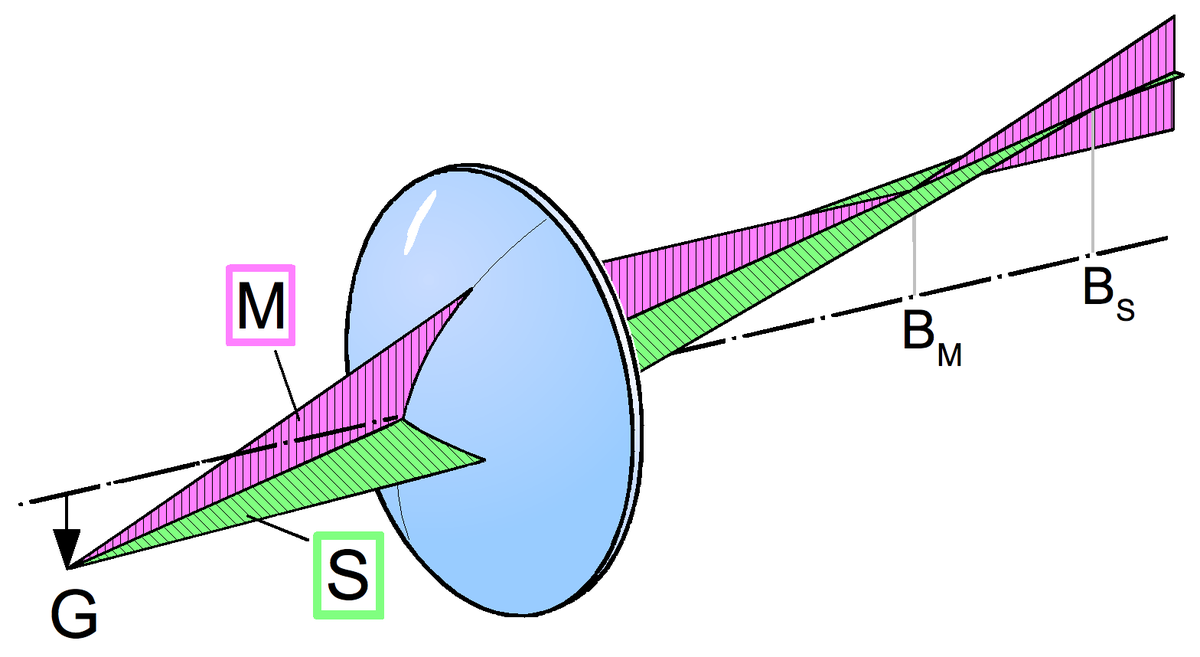
\includegraphics[width=.5\textwidth]{img/astigmatismo.png}

\caption{Astigmatismo}
\label{fig:astigmatismo}
\end{figure}

\subsection{Curvatura di campo}
La curvatura di campo è un'aberrazione
monocromatica extra assiale coniugata all'astigmatismo dei fasci obliqui.
Nonostante l'eliminazione dell'astigmatismo dei fasci obliqui, l'immagine di
un oggetto piano, che sia perpendicolare all'asse ottico, si forma comunque su
una superficie curva, la superficie di Petzval. La deviazione indotta dal
piano immagine viene quindi definita curvatura di campo.

\begin{figure}

\centering
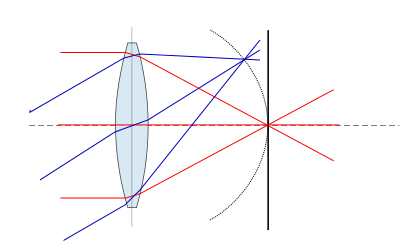
\includegraphics[width=.5\textwidth]{img/curvatura-campo.png}

\caption{Curvatura di campo}
\label{fig:curvatura-campo}
\end{figure}

\subsection{Distorsione}
In ottica geometrica la distorsione è la deviazione da una proiezione rettilinea, una proiezione in cui le rette nella scena rimangono rette nel piano dell'immagine.
Nonostrante la distorsione possa essere irregolare, la condizione che si verifica più frequente è la distorsione radiale simmetrica, solitamente esse vengono classificate come \emph{a cuscino}, \emph{a barile}.

\paragraph{Distorsione a cuscino:}
L'ingrandimento dell'immagine cresce con la distanza dall'asse ottico, l'effetto visibile è che le line che non passano per il centro dell'èimagine sono piegate verso il centro dell' immagine.
\paragraph{Distorsione a barile:}
L'ingrandimento diminuisce con la distanza dall'asse ottico, l'effetto apparente è che l'immagine sembra mappata su di una sfera, lenti grandangolari utilizzano questo tipo di distorsione per mappare un oggetto infinitamente largo in un area finita.
\begin{figure}[!h]
\begin{subfigure}[b]{.5\textwidth}
\centering
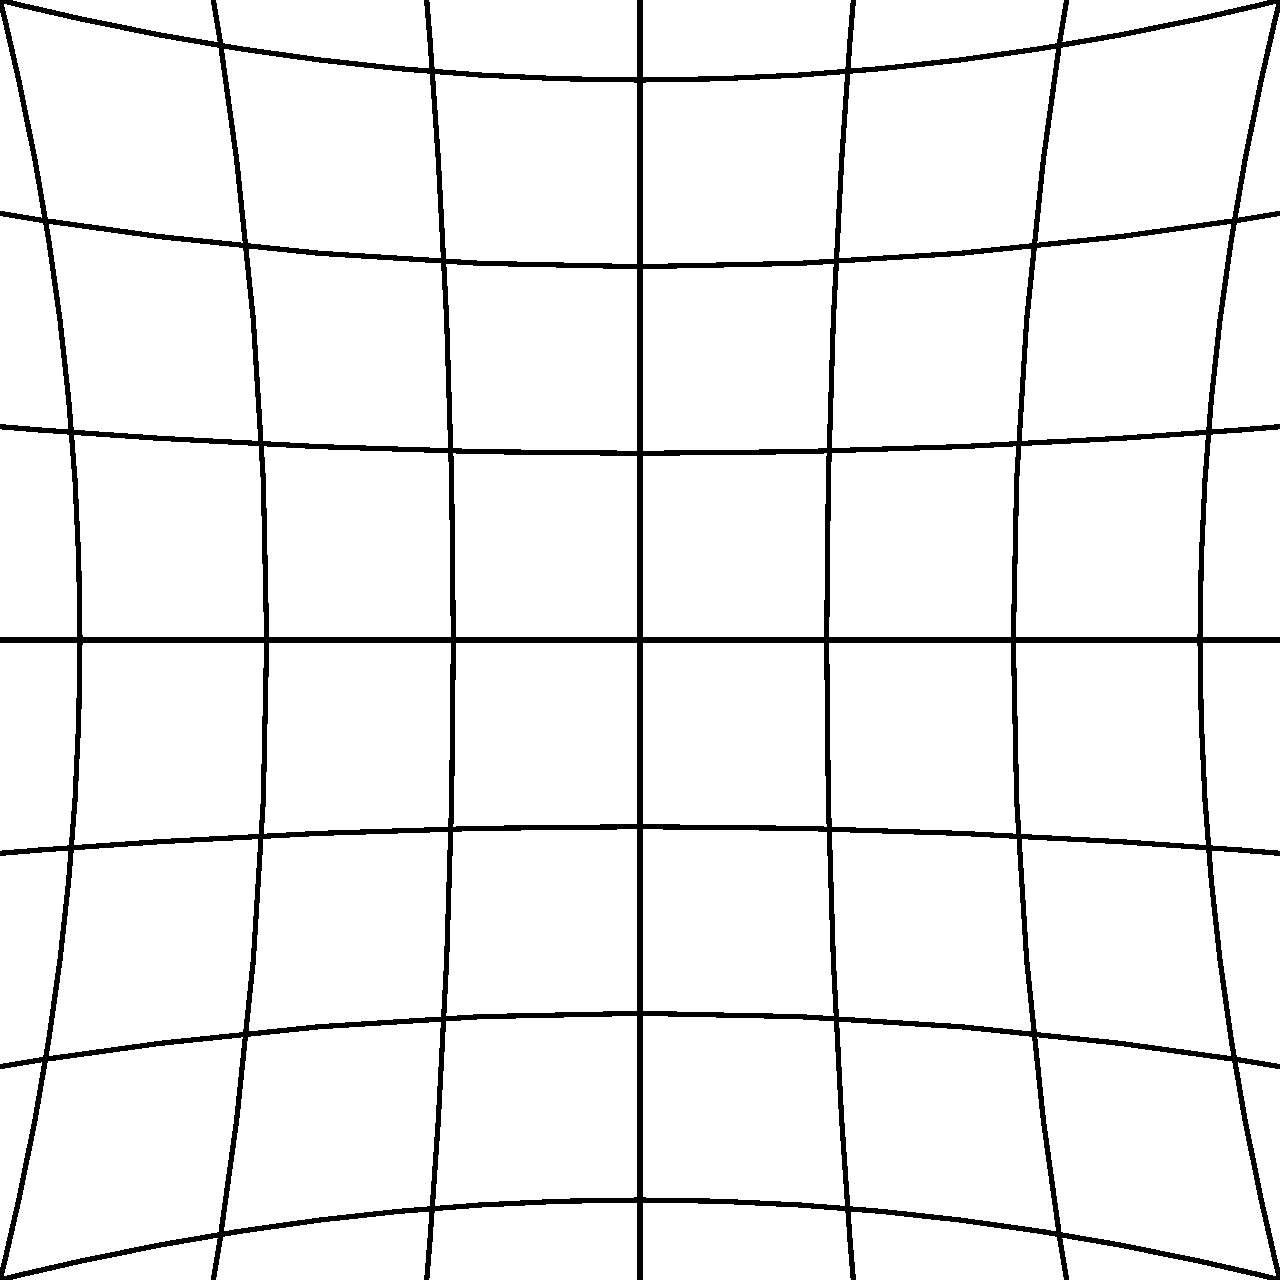
\includegraphics[height=3cm]{img/distorsione-cuscino.pdf}
\caption{Cuscino}\label{fig:distorsione-cuscino}
\end{subfigure}
\begin{subfigure}[b]{.5\textwidth}
\centering
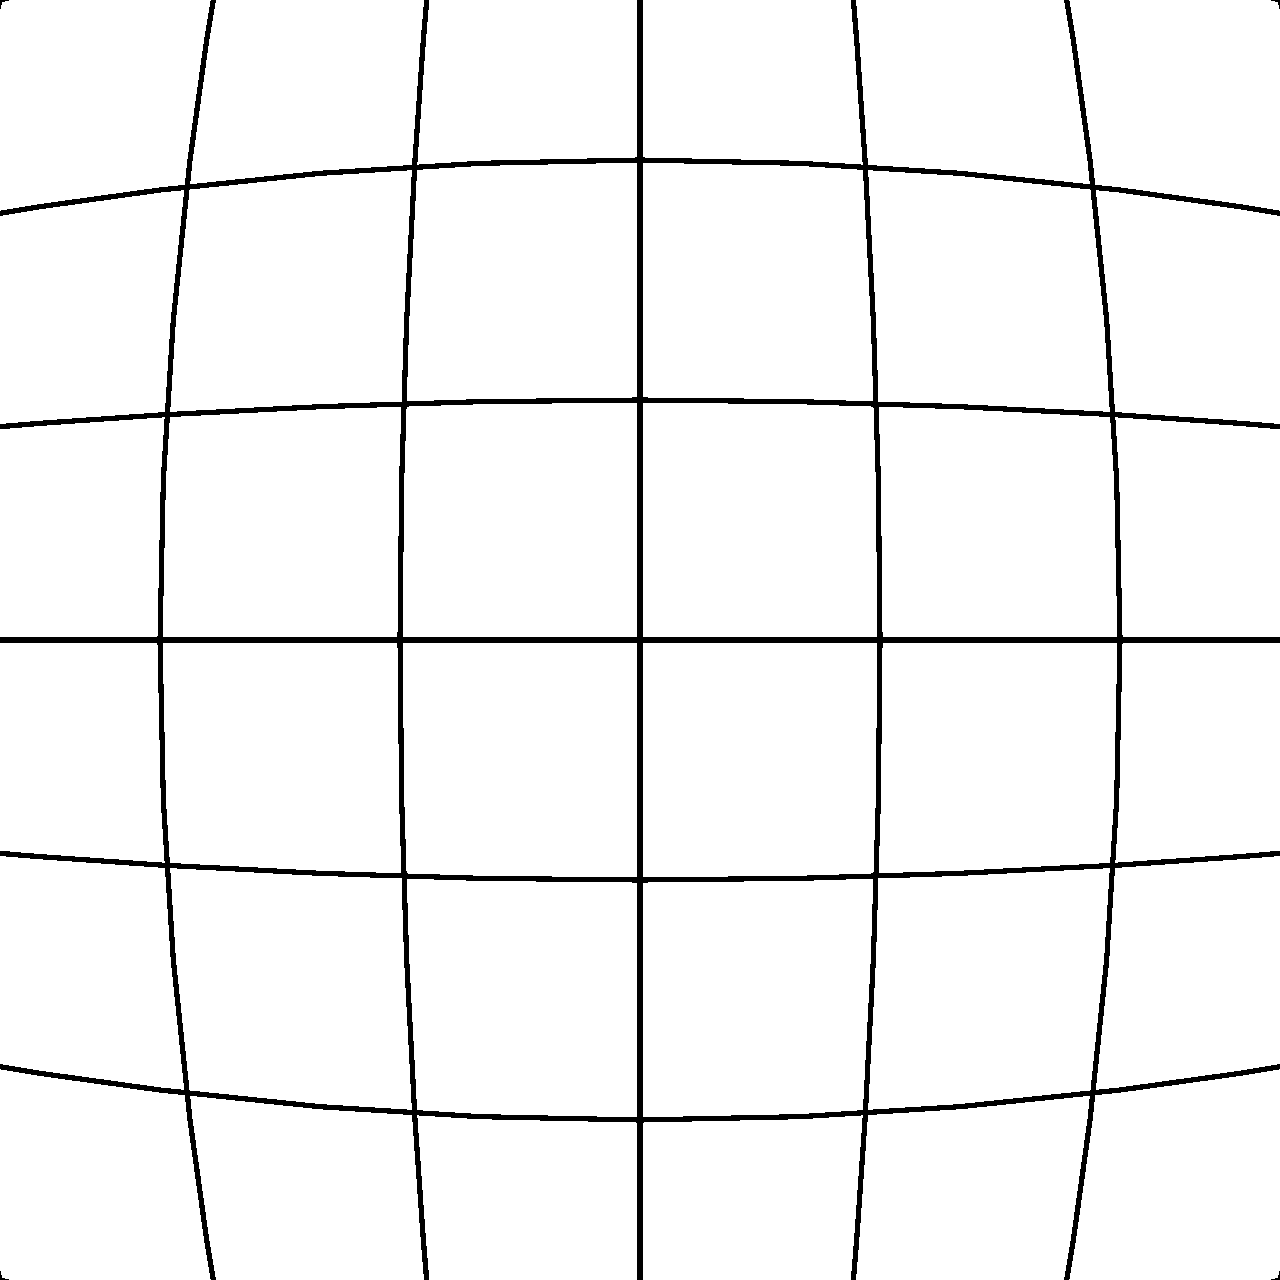
\includegraphics[height=3cm]{img/distorsione-barile.pdf}
\caption{Barile}\label{fig:distorsione-barile}
\end{subfigure}
\caption{Distorsione}
\label{fig:distorsione}
\end{figure}

Essendo la distorsione radiale principalmente dominata da componenti radiali di basso ordine[CITAZIONE], possono essere corrette usando il modello di distorsione di Brown, esso corregge sia le distorsioni radiali che quelle tangenziali causate dall'impreciso allineamento delle lenti.
 %Citazione de Villiers, J. P.; Leuschner, F.W.; Geldenhuys, R. (17–19 November 2008). "Centi-pixel accurate real-time inverse distortion correction". "2008 International Symposium on Optomechatronic Technologies". SPIE. doi:10.1117/12.804771.

\[
 x_\mathrm{d} = x_\mathrm{u}(1 + K_1r^2 + K_2r^4 + \cdots) + 
(P_2(r^2 + 2x_\mathrm{u}^2) + 2P_1 x_\mathrm{u}y_\mathrm{u})(1 + P_3r^2 + P_4r^4 \cdots) \]

\[y_\mathrm{d} = y_\mathrm{u}(1 + K_1r^2 + K_2r^4 + \cdots) + 
(P_1(r^2 + 2y_\mathrm{u}^2) + 2P_2 x_\mathrm{u}y_\mathrm{u})(1 + P_3r^2 + P_4r^4 \cdots)
\]

\begin{itemize}

\item $(x_\mathrm{d},\ y_\mathrm{d})$=  Punti distorti proiettati sul piano immaginespecified lens;
\item $(x_\mathrm{u},\ y_\mathrm{u})$ = Punti non distorti proiettati da una camera pinhole ideale;
\item $(x_\mathrm{c},\ y_\mathrm{c})$ = Centro di distorsione;
\item $K_n = n^{\mathrm{th}}$ = Coefficienti di distorsione radiale;
\item $P_n = n^{\mathrm{th}}$ = Coefficienti di distorsione tangenziale;
\item $r = \sqrt{(x_\mathrm{u}-x_\mathrm{c})^2 + (y_\mathrm{u}-y_\mathrm{c})^2}$
\end{itemize}


\subsection{Aberrazione cromatica}

Una lente singola non è soddisfacente come obbiettivo perché l'indice di rifrazione, da
cui dipende la lunghezza focale, è diverso a seconda della lunghezza d'onda della luce, cioé del suo
colore. In pratica, la luce rossa viene focalizzata più lontano, la luce blu più vicino, e quindi non c'è
un ben definito piano dell'immagine (Figura \ref{fig:aberrazione-cromatica}). Tale caratteristica del vetro è definita dispersione
ed è sempre presente, anche se in modo diverso da vetro a vetro. La soluzione a questo problema sta
nel combinare due lenti di vetri diversi, scelti in modo che il risultato porti a una compensazione. Di solito si combina una lente convergente con bassa dispersione (vetro crown) con una lente divergente con alta dispersione (vetro flint). Il sistema rimane sempre convergente, perché la lente divergente è meno potente di quella convergente, tuttavia la sua maggior dispersione compensa quella di verso opposto introdotta dalla lente convergente. Questa combinazione viene detta doppietto acromatico (Figura \ref{fig:doppietto-acromatico}). La correzione, per quanto buona, non è perfetta, e può essere migliorata usando vetri speciali molto costosi in combinazioni di due lenti (doppietti) o tre (tripletti). In tal caso gli obbiettivi vengono detti apocromatici.



\begin{figure}

\centering
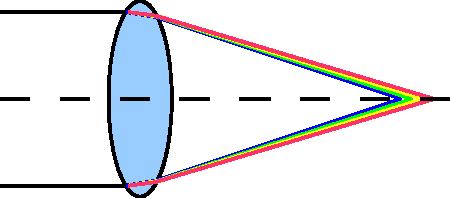
\includegraphics{img/aberrazione-cromatica.pdf}

\caption{Aberrazione cromatica}
\label{fig:aberrazione-cromatica}
\end{figure}


\begin{figure}

\centering
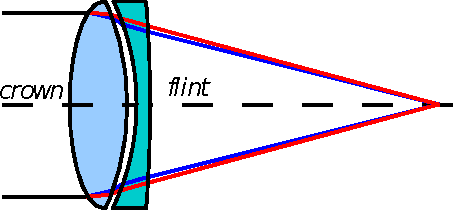
\includegraphics{img/doppietto-acromatico.pdf}

\caption{Doppietto acromatico}
\label{fig:doppietto-acromatico}
\end{figure}

\subsection{Ingrandimento e luminosità}

La dimensione dell'immagine formata nel piano focale dipende dalla lunghezza
focale e, ovviamente, dalla dimensione dell'oggetto che si osserva. Se
l'angolo sotteso dall'oggetto è $\theta$, allora la dimensione sul piano
focale è: 
\[l = f tan(\theta)\]
Per piccoli angoli la tangente si può approssimare con l'argomento
\[\lim_{\theta \to 0} tan(\theta) = \theta \]
quindi 
\[l \simeq f \cdot \theta\]
La quantità di luce raccolta da un obbiettivo,dipende dalla sua area, cioé da 
\[A=\frac{\pi}{4} \cdot d^2\]
dove $d$ è il diametro dell'obiettivo
Se puntiamo un obbiettivo contro un oggetto esteso la quantità di luce raccolta sarà proporzionale a $d^2$,
ma l'ingrandimento farà sì che questa luce venga sparsa su un'area proporzionale al quadrato della lunghezza focale $f^2$ .
\[A=\frac{\pi}{4} \cdot \left(\frac{d}{f}\right)^2 \]
Quindi la luminosità superficiale dell'immagine sarà proporzionale a $\left(\frac{d}{f}\right)^2 $
\\
Il rapporto 
\[ f/\# = \frac{f}{d} \] 
viene chiamato rapporto focale ed indica la luminosità di un obbiettivo (telescopico o fotografico).

Ad esempio, un telescopio da 100\unit{mm} di diametro e 1000\unit{mm} di focale ha un rapporto $f/d$ pari a 10 (indicato con
$1:10$, oppure $f/10$). Un telescopio da 100\unit{mm} di diametro e 500\unit{mm} di focale, invece, ha un rapporto
$f/d$  pari a 5 (indicato con $1:5$ oppure $f/5$), ed è più luminoso, cioè l'immagine sul piano focale avrà
una luminosità superficiale più alta.

\subsection{La risoluzione}